%% JEPA-Reg — ICCA 2026 camera-ready revision (Paper 284)
%% Template: ACM acmart, sigconf (per ICCA_2026_LaTex_Template)
%% TODO before camera-ready upload:
%%   1. Replace \acmDOI and \acmISBN below with the values from your ACM rights form.
%%   2. Confirm the author block against the ACM rights confirmation email.
%%   3. Regenerate figures 2, 3, 4, 5 and 6 (see FIGURE NOTE comments in the body).
\documentclass[sigconf]{acmart}

%% Keep floats within their own sections (prevents figures/tables drifting
%% into the following section).
\usepackage{placeins}
\usepackage{dblfloatfix}
%% \usepackage{flafter}  %% removed: it defers wide floats and opens vertical gaps
%% Algorithm 1 (Section 3.4). If your TeX distribution reports a clash here,
%% swap these two lines for: \usepackage[ruled,vlined]{algorithm2e}
\usepackage{algorithm}
\usepackage{algpseudocode}

%% Float placement parameters: the defaults are conservative enough that a page
%% carrying one full-width table can be rejected outright, which shows up as a
%% large band of white space.
\renewcommand{\topfraction}{0.9}
\renewcommand{\dbltopfraction}{0.9}
\renewcommand{\bottomfraction}{0.7}
\renewcommand{\textfraction}{0.07}
\renewcommand{\floatpagefraction}{0.75}
\renewcommand{\dblfloatpagefraction}{0.75}
\setcounter{topnumber}{3}
\setcounter{dbltopnumber}{3}
\setcounter{totalnumber}{5}

\AtBeginDocument{%
  \providecommand\BibTeX{{Bib\TeX}}}

\setcopyright{acmlicensed}
\copyrightyear{2026}
\acmYear{2026}
%% TODO: replace with the DOI from your ACM rights form
\acmDOI{XXXXXXX.XXXXXXX}
\acmConference[ICCA 2026]{the 4th International Conference on Computing Advancements}{October 15--16, 2026}{Dhaka, Bangladesh}
%% TODO: replace with the ISBN from your ACM rights form
\acmISBN{978-1-4503-XXXX-X/2026/10}

\begin{document}

\title[JEPA-Reg for Robust Paraphrase Detection]{JEPA-Reg: Predictive Representation Regularization Improves Robustness to Adversarial Lexical Overlap in Paraphrase Detection}

\author{Saeef Uddin Ahmed}
\affiliation{%
  \department{Department of Computer Science}
  \institution{American International University-Bangladesh (AIUB)}
  \city{Dhaka}
  \country{Bangladesh}
}
\email{25-93814-2@student.aiub.edu}

\author{Irtiza Ahsan Abir}
\affiliation{%
  \department{Department of Computer Science}
  \institution{American International University-Bangladesh (AIUB)}
  \city{Dhaka}
  \country{Bangladesh}
}
\email{25-93739-2@student.aiub.edu}

\author{Sandip Misra}
\affiliation{%
  \department{Department of Computer Science}
  \institution{American International University-Bangladesh (AIUB)}
  \city{Dhaka}
  \country{Bangladesh}
}
\email{25-93890-3@student.aiub.edu}

\author{Mehedi Hasan Rudro}
\affiliation{%
  \department{Department of Computer Science}
  \institution{American International University-Bangladesh (AIUB)}
  \city{Dhaka}
  \country{Bangladesh}
}
\email{26-93945-1@student.aiub.edu}

%% Final Author (Research Supervisor)
\author{Abdus Salam}
\affiliation{%
  \department{Department of Computer Science}
  \institution{American International University-Bangladesh (AIUB)}
  \city{Dhaka}
  \country{Bangladesh}
}
\email{abdus.salam@aiub.edu}

\begin{abstract}
Paraphrase detection models trained on standard benchmarks over-rely on superficial lexical overlap, resulting in performance drops on adversarial datasets such as PAWS and HANS. We propose \textbf{JEPA-Reg}, a lightweight regularization approach that augments BERT-based paraphrase classifiers with a Joint-Embedding Predictive Architecture (JEPA) auxiliary loss. An exponential-moving-average (EMA) target encoder with stop-gradient provides stable prediction targets, and, unlike prior JEPA variants, the predictive loss is applied only to labeled paraphrase pairs, giving the encoder a label-conditioned inductive bias toward structurally grounded, overlap-invariant representations without negative sampling or cross-modal data construction. We evaluate on MRPC, QQP, and PAWS with three random seeds. When fine-tuning on PAWS, JEPA-Reg improves BERT-base test F1 by +7.9 points (71.7$\rightarrow$79.6) and reduces seed-to-seed standard deviation by 15$\times$ (3.74$\rightarrow$0.24); for RoBERTa-base the mean gain is small (+0.22) but seed-consistent. Stratifying PAWS accuracy by lexical overlap quartile shows JEPA-Reg's largest advantage in the highest-overlap quartile and gains on both classes, indicating reduced reliance on surface co-occurrence rather than a shifted class prior. In zero-shot transfer to HANS, JEPA-Reg improves overall F1 (+3.0), but a per-subcase analysis reveals this stems chiefly from a shift in prediction bias, which we report as a negative result for the structural-transfer hypothesis. Because only three seeds are used, we report per-seed values and effect sizes descriptively rather than claiming small $p$-values. JEPA-Reg adds no inference-time cost and is conceived as a targeted adversarial-robustness regularizer rather than a general accuracy booster: on QQP it neither helps nor hurts (76.7$\pm$0.3 vs.\ 76.3$\pm$0.8).
\end{abstract}

\begin{CCSXML}
<ccs2012>
 <concept>
  <concept_id>10010147.10010178.10010179</concept_id>
  <concept_desc>Computing methodologies~Natural language processing</concept_desc>
  <concept_significance>500</concept_significance>
 </concept>
 <concept>
  <concept_id>10010147.10010257.10010258.10010259</concept_id>
  <concept_desc>Computing methodologies~Supervised learning by classification</concept_desc>
  <concept_significance>300</concept_significance>
 </concept>
 <concept>
  <concept_id>10010147.10010257.10010293.10010294</concept_id>
  <concept_desc>Computing methodologies~Neural networks</concept_desc>
  <concept_significance>300</concept_significance>
 </concept>
</ccs2012>
\end{CCSXML}

\ccsdesc[500]{Computing methodologies~Natural language processing}
\ccsdesc[300]{Computing methodologies~Supervised learning by classification}
\ccsdesc[300]{Computing methodologies~Neural networks}

\keywords{Paraphrase detection, Adversarial robustness, Lexical overlap, JEPA, Representation learning, Natural language processing}

\maketitle

\section{Introduction}
Pre-trained transformer models such as BERT~\cite{devlin2019bert} and RoBERTa~\cite{liu2019roberta} perform well on paraphrase-detection benchmarks such as MRPC and QQP in the GLUE suite~\cite{wang2019glue}. However, a well-documented failure mode is their dependence on lexical-overlap heuristics: models tend to predict ``paraphrase'' when token overlap is high, even when syntactic structure indicates otherwise~\cite{mccoy2019right}. Datasets such as PAWS~\cite{zhang2019paws} and HANS~\cite{mccoy2019right} expose this behavior by creating adversarial sentence pairs with high lexical overlap but conflicting labels.

Current mitigation options have significant limitations. Adversarial fine-tuning methods, e.g., SMART~\cite{jiang2020smart} and FreeLB~\cite{zhu2020freelb}, and regularization methods, e.g., Mixout~\cite{lee2020mixout}, improve general robustness but do not explicitly address lexical-overlap reliance. Debiasing methods~\cite{clark2019dont,utama2020towards} assume the bias is known a priori. Contrastive learning methods such as SimCSE~\cite{gao2021simcse}, DeCLUTR~\cite{giorgi2021declutr}, and INSTRUCTOR~\cite{su2023instructor} enhance representation quality but depend on explicit negative-pair construction and are not built to directly address structural robustness under adversarial overlap.

An alternative framework for learning representations is given by JEPA. I-JEPA~\cite{assran2023ijepa} trains an online encoder to predict the representations of an EMA target encoder in embedding space, without negative samples or heavy augmentations. LLM-JEPA~\cite{huang2025llmjepa} extends this to large language models with cross-modal views, but works mainly in generative settings. To our knowledge, JEPA has not previously been employed for adversarial robustness in encoder-based discriminative classification.

\textbf{Contributions.} We introduce JEPA-Reg and make the following contributions, whose novelty relative to prior JEPA work we make explicit:
\begin{itemize}
\item \textbf{Method.} We adapt the JEPA predictive-EMA objective to same-modality sentence pairs in a \emph{discriminative} setting, and, departing from all prior JEPA variants---which apply the predictive loss to every view pair---we \textbf{condition the auxiliary loss on the gold label}, applying it only to annotated paraphrase pairs. This makes the auxiliary signal task-aligned by design: semantically equivalent sentences must be mutually predictable in projection space, while non-paraphrases are exempt. (An ablation in Section~\ref{sec:maskablation} shows the unmasked variant performs comparably on PAWS, so we present label conditioning as a principled design choice rather than the empirical source of the gains.)
\item \textbf{Empirical findings.} On PAWS fine-tuning, JEPA-Reg yields both a mean F1 gain (+7.9 for BERT-base) and a 15$\times$ reduction in seed-to-seed standard deviation, with the largest advantage in the most overlap-heavy stratum.
\item \textbf{Analysis.} We provide the first systematic multi-seed study of the auxiliary-loss weight $\lambda$ for JEPA in NLP classification, finding, contrary to single-run evidence, that the method's robustness gain is insensitive to $\lambda$ across $[0.05, 1.0]$, so no careful tuning away from the LLM-JEPA default is required.
\item \textbf{Honest negative results.} We report per-subcase HANS diagnostics showing that zero-shot heuristic-level gains reflect prediction-bias shifts rather than transferred structural reasoning, and an STS-B diagnostic bounding the method's scope to classification.
\end{itemize}

\textbf{Scope.} JEPA-Reg is conceived as a targeted adversarial-robustness regularizer, not a general-purpose accuracy booster. On large, clean datasets like QQP, which do not exhibit strong overlap--label dissociation, it neither helps nor hurts (Section~\ref{sec:qqp}).

\section{Literature Review}
The lexical-overlap failure is most clearly instantiated by PAWS~\cite{zhang2019paws}, which builds adversarial pairs with high lexical overlap but different labels via controlled word reordering, and HANS~\cite{mccoy2019right}, which decomposes the problem into lexical overlap, subsequence, and constituent heuristics. Together these benchmarks establish that lexical-overlap bias is a representation-level phenomenon and motivate methods that intervene directly on how models construct internal representations.

Three families of prior work address related problems. \emph{Adversarial fine-tuning}---SMART~\cite{jiang2020smart}, which uses Bregman proximal perturbations in embedding space, and FreeLB~\cite{zhu2020freelb}, which accumulates iterative gradient-based perturbations---improves general robustness but perturbs inputs uniformly without specifically targeting lexical-overlap reliance; Mixout~\cite{lee2020mixout} stochastically interpolates fine-tuned parameters with pre-trained ones to guard against catastrophic forgetting, but introduces no structural inductive bias. \emph{Debiasing methods}~\cite{clark2019dont,utama2020towards} employ auxiliary biased models or product-of-experts formulations; they are the natural comparators for overlap shortcuts and are computationally cheap at the 110M scale, so we identify them as the priority baseline for future comparison (Section~\ref{sec:limitations}). \emph{Contrastive representation learning}---Sentence-BERT~\cite{reimers2019sentencebert}, SimCSE~\cite{gao2021simcse}, DeCLUTR~\cite{giorgi2021declutr}, INSTRUCTOR~\cite{su2023instructor}---is inherently dependent on explicit negative-pair construction, resulting in sensitivity to batch composition, and optimizes general semantic similarity rather than structural robustness under adversarial overlap.

Negative-free self-supervised techniques from vision, such as Barlow Twins~\cite{zbontar2021barlow} and BYOL~\cite{grill2020byol}, show that discriminative representations can be learned without negatives but have not been applied to discriminative NLP tasks. I-JEPA~\cite{assran2023ijepa} trains an online encoder to predict embeddings of masked target patches via an EMA-updated target encoder, entirely in representation space; DINO~\cite{caron2021dino} and data2vec~\cite{baevski2022data2vec} further validate EMA self-distillation across modalities. LLM-JEPA~\cite{huang2025llmjepa} extends JEPA to decoder-only LLMs with cross-modal text--code views, and VL-JEPA~\cite{chen2025vljepa} to vision--language learning. None of this work applies JEPA to same-modality sentence pairs in a discriminative setting.

Structural probing~\cite{hewitt2019structural,tenney2019bert} shows that BERT layers encode rich syntactic information, yet fine-tuning pressures that reward lexical shortcuts suppress this structural knowledge in final predictions. Data augmentation via back-translation~\cite{sennrich2016improving} and EDA~\cite{wei2019eda} broadens the training distribution but leaves lexical sensitivity unchanged. Output-level regularizers such as R-Drop~\cite{wu2021rdrop} operate at the logit level with no geometric constraint on the representation space where overlap heuristics form.

Table~\ref{tab:related} compares methods on four \emph{method-property} criteria: (i) requires no negative sampling; (ii) imposes a geometric constraint directly on the representation space; (iii) operates on same-modality inputs without auxiliary bias models or cross-modal views; (iv) conditions its objective on task labels. No prior JEPA work evaluates on adversarial overlap benchmarks or studies $\lambda$ in a discriminative setting.

\begin{table}[!htbp]
\caption{Comparison of related methods by key properties.}
\label{tab:related}
\begin{tabular}{lcccc}
\toprule
Method & Neg.-free & Repr.\ constr. & Same-mod. & Label-cond. \\
\midrule
SMART / FreeLB & \checkmark & $\times$ & \checkmark & $\times$ \\
Mixout & \checkmark & $\times$ & \checkmark & $\times$ \\
Debiasing & \checkmark & $\times$ & $\times$ & \checkmark \\
SimCSE / DeCLUTR & $\times$ & \checkmark & \checkmark & $\times$ \\
Barlow Twins / BYOL & \checkmark & \checkmark & \checkmark & $\times$ \\
I-JEPA / LLM-JEPA & \checkmark & \checkmark & $\times$ & $\times$ \\
\textbf{JEPA-Reg (ours)} & \checkmark & \checkmark & \checkmark & \checkmark \\
\bottomrule
\end{tabular}
\end{table}

\section{Method: JEPA-Reg}

\subsection{Problem Formulation and Overview}
Let $f_\theta$ denote a BERT-based encoder and $(s_1, s_2, y)$ a training triple with $y \in \{0,1\}$. Standard fine-tuning minimizes
\begin{equation}
L_{\mathrm{cls}} = \mathrm{CrossEntropy}\big(W \cdot \mathrm{pool}(f_\theta(\mathrm{tok}(s_1, s_2))),\, y\big),
\label{eq:cls}
\end{equation}
%% TODO (author check): the submitted text said the baseline used "the standard
%% classification head of the pretrained architecture", which conflicts with the
%% mean-pooling definition above. The sentence below assumes mean pooling is used in
%% BOTH conditions. If the baseline in fact used the pretrained [CLS] pooler head,
%% replace the second sentence with an explicit statement of that difference.
where $\mathrm{pool}(\cdot)$ is attention-masked \emph{mean pooling} over the final hidden states of the cross-encoded pair. The same pooling and classification head are used for the baseline and for JEPA-Reg, so the two conditions differ only in the auxiliary loss and in label smoothing (Section~\ref{sec:limitations}). JEPA-Reg adds a representation-level auxiliary loss to Eq.~(\ref{eq:cls}). The complete training pipeline is depicted in Figure~\ref{fig:workflow}.

\begin{figure}[!htbp]
  \centering
  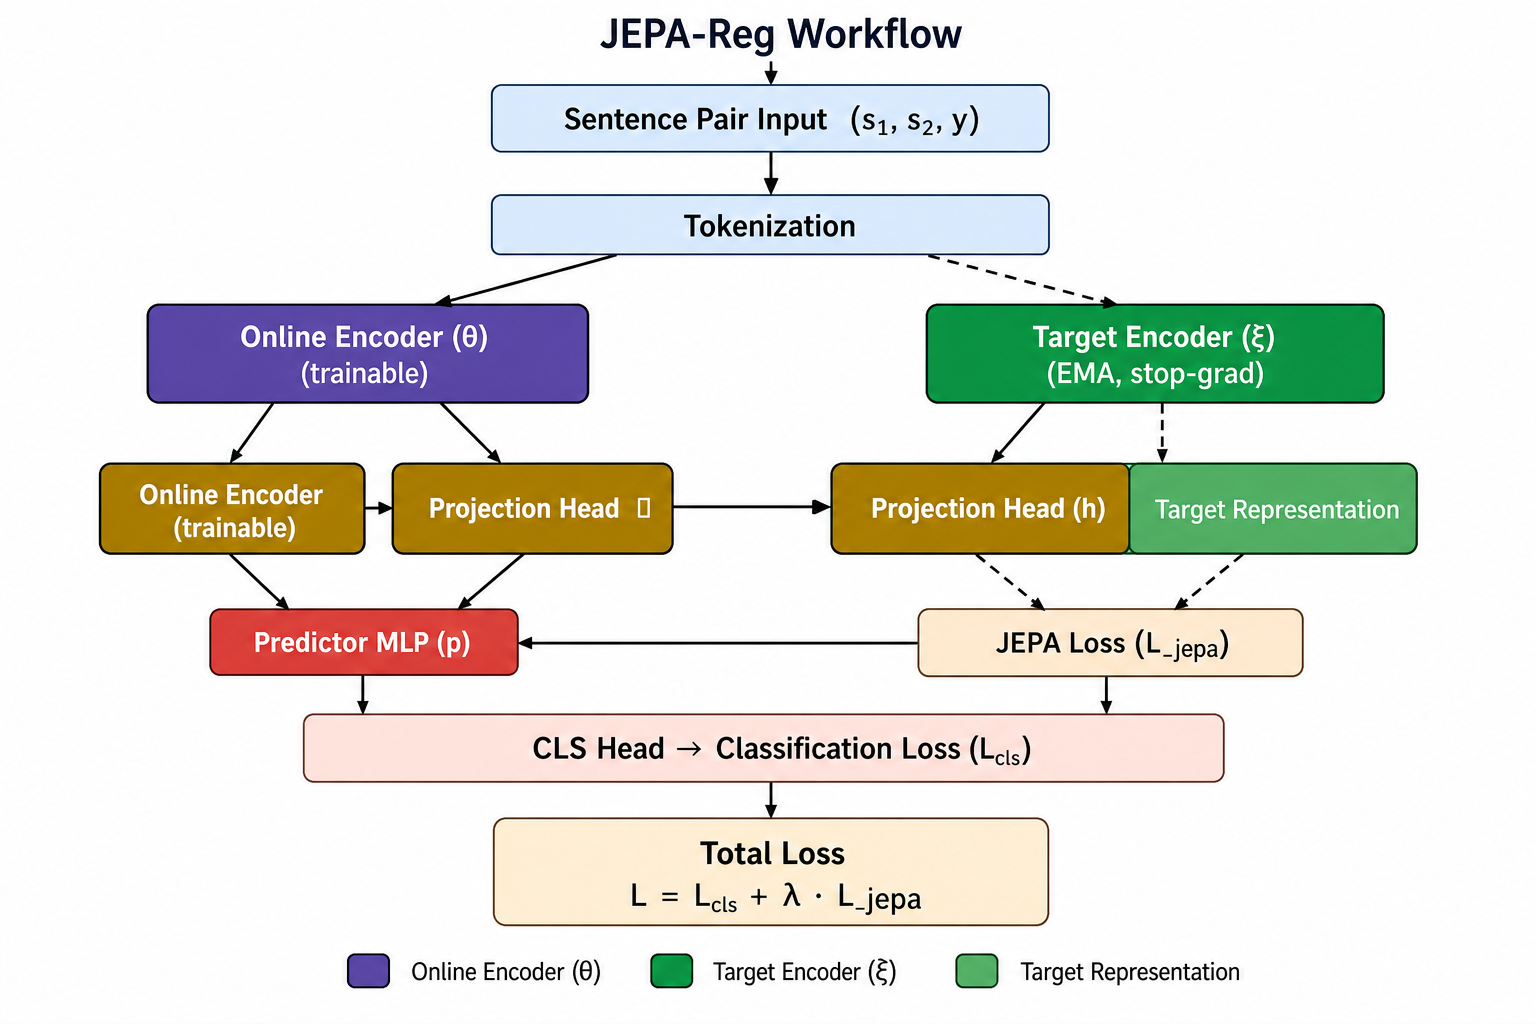
\includegraphics[width=\linewidth]{figs/fig1_workflow}
  %% FIGURE NOTE: if this figure still shows two separate "Online Encoder" boxes,
  %% label them distinctly (cross-encoded pair vs. individually encoded s1, s2) and
  %% either complete the color legend or remove it -- it currently covers only three
  %% of the six colors used.
  \caption{JEPA-Reg training pipeline: data and loss flow from the input pair to the total objective. Figure~\ref{fig:arch} gives the corresponding gradient and EMA flow.}
  \Description{Flow diagram: a sentence pair is tokenized and passed to a trainable online encoder and an EMA target encoder with stop-gradient; projection heads and a predictor MLP produce the JEPA loss, combined with the classification loss into the total loss.}
  \label{fig:workflow}
\end{figure}

\subsection{Dual-Encoder Architecture}
JEPA-Reg maintains two encoders with identical architecture but different update rules. The online encoder $f_\theta$ is fully trainable and receives gradients from both losses. The target encoder $f_\xi$ is a non-trainable copy updated as an exponential moving average:
\begin{equation}
\xi \leftarrow \tau\xi + (1-\tau)\theta, \quad \tau = 0.999.
\label{eq:ema}
\end{equation}
Stop-gradient is applied only to the target branch: the online encoder receives the full JEPA gradient through the predictor and projection head, while the target provides a stable reference, consistent with I-JEPA~\cite{assran2023ijepa}. Figure~\ref{fig:arch} summarizes the gradient flow. Both branches use a projection head of the same architecture $h$: $\mathrm{Linear}(H{\to}H) \to \mathrm{GELU} \to \mathrm{Linear}(H{\to}256)$; the target-side copy $h_\xi$ is EMA-updated together with $f_\xi$ by Eq.~(\ref{eq:ema}), and the online branch adds a predictor $p$ of the same structure. For each sentence $s_i$ (encoded \emph{individually}, not as a pair):
\begin{equation}
z_i = h(\mathrm{pool}(f_\theta(s_i))), \qquad \tilde{z}_i = h_\xi(\mathrm{pool}(f_\xi(s_i))).
\label{eq:proj}
\end{equation}

\begin{figure}[!htbp]
  \centering
  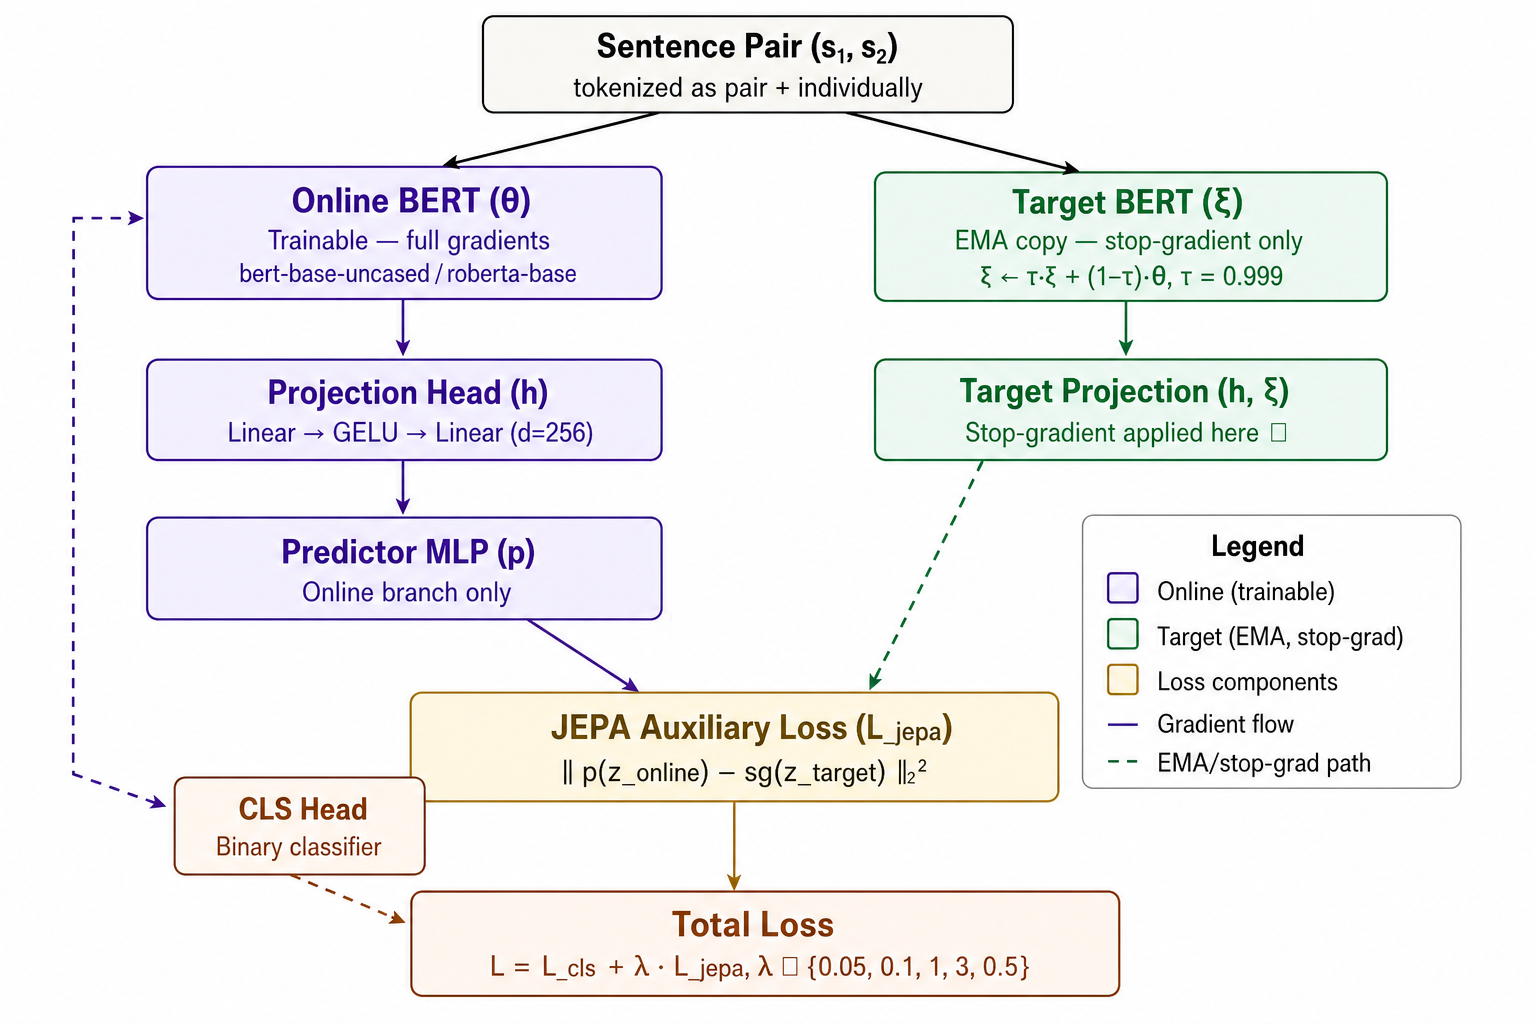
\includegraphics[width=\linewidth]{figs/fig2_architecture}
  %% FIGURE NOTE: three corrections needed in the image itself --
  %%   (a) the lambda set renders as {0.05, 0.1, 1, 3, 0.5}; it must read {0.05, 0.1, 0.3, 0.5};
  %%   (b) the loss box shows ||p(z_online) - sg(z_target)||^2 without the normalization
  %%       hats, which states a different objective from Eq. (4) -- use the hatted form
  %%       or write the cosine form;
  %%   (c) relabel "CLS Head" as "Classifier Head" to match the mean pooling in Sec. 3.1.
  \caption{Dual-encoder JEPA-Reg architecture: gradient flow (online branch) and EMA target updates under stop-gradient.}
  \Description{Architecture diagram showing the online encoder receiving gradients from both the classification loss and the JEPA loss, while the target encoder receives only EMA updates under stop-gradient.}
  \label{fig:arch}
\end{figure}

\subsection{JEPA Auxiliary Loss (Label-Conditioned)}
\label{sec:loss}
All projections are $\ell_2$-normalized; writing $\hat{u} = u / \lVert u \rVert_2$, the symmetric predictive loss for one pair is
\begin{equation}
\ell(s_1, s_2) = \tfrac{1}{2}\Big[\big(1 - \hat{p}(z_1)^\top \hat{\tilde z}_2\big) + \big(1 - \hat{p}(z_2)^\top \hat{\tilde z}_1\big)\Big],
\label{eq:pairloss}
\end{equation}
a cosine-distance form equivalent (up to a factor of 2) to the squared-$\ell_2$ distance between normalized vectors. The auxiliary loss is applied \emph{only to gold paraphrase pairs}:
\begin{equation}
L_{\mathrm{jepa}} = \frac{\sum_n \mathbb{1}[y^{(n)}{=}1]\; \ell(s_1^{(n)}, s_2^{(n)})}{\max\big(1, \sum_n \mathbb{1}[y^{(n)}{=}1]\big)}.
\label{eq:jepa}
\end{equation}
This label conditioning is the theoretically motivated choice: mutual predictability in latent space is justified for semantically equivalent sentences, whereas forcing labeled non-paraphrases toward mutual predictability would directly oppose the classification objective. Section~\ref{sec:maskablation} ablates this choice against the unmasked (all-pairs, BYOL-style) variant and includes a representation-collapse check. Because the objective is defined entirely in embedding space, it imposes no pressure to reconstruct input tokens.

\subsection{Full Objective and Computational Cost}
\label{sec:objective}
\begin{equation}
L = L_{\mathrm{cls}} + \lambda\, L_{\mathrm{jepa}}.
\label{eq:full}
\end{equation}
$\lambda$ is selected on a 10\% held-out fraction of the \emph{training} set (disjoint from the QQP test split described in Section~\ref{sec:datasets}, which is also carved out at 10\%) from candidates $\{0.05, 0.1, 0.3, 0.5\}$ using a single tuning seed and one epoch; this held-out selection chooses $\lambda=0.05$ for BERT-base on all three datasets (for RoBERTa-base we fix $\lambda=0.1$ without a sweep). The subsequent three-seed test-set sensitivity study in Section~\ref{sec:lambda} is a separate experiment batch and should not be interpreted as a replication of the main-results checkpoints; its purpose is to assess sensitivity to $\lambda$, not to select $\lambda$ by test F1. To stabilize early training, $\lambda$ is warmed up linearly from 0 to its target value over the first epoch. Algorithm~\ref{alg:jepareg} summarizes the complete training procedure.

\begin{algorithm}[!tb]
\caption{JEPA-Reg training}
\label{alg:jepareg}
\begin{algorithmic}[1]
\Require Training pairs $\{(s_1^{(n)}, s_2^{(n)}, y^{(n)})\}$; weight $\lambda$; EMA decay $\tau=0.999$
\State Initialize $f_\theta$; set $f_\xi \leftarrow f_\theta$; initialize heads $h$, $h_\xi \leftarrow h$, $p$, classifier $W$
\For{each minibatch $B$}
  \State $z_i \leftarrow h(\mathrm{pool}(f_\theta(s_i)))$ \Comment{online, grad}
  \State $\tilde{z}_i \leftarrow \mathrm{sg}\big(h_\xi(\mathrm{pool}(f_\xi(s_i)))\big)$ \Comment{target, Eq.~(\ref{eq:proj})}
  \State $L_{\mathrm{cls}} \leftarrow \mathrm{CrossEntropy}\big(W \cdot \mathrm{pool}(f_\theta(\mathrm{tok}(s_1,s_2))), y\big)$
  \State $L_{\mathrm{jepa}} \leftarrow$ mean of $\ell(s_1,s_2)$ over $\{n \in B : y^{(n)}{=}1\}$ \Comment{Eq.~(\ref{eq:jepa})}
  \State $\lambda_{\mathrm{eff}} \leftarrow \lambda \cdot \min(1, \text{step}/\text{steps per epoch})$ \Comment{warmup}
  \State Update $\theta$ using $\nabla_\theta\big(L_{\mathrm{cls}} + \lambda_{\mathrm{eff}} L_{\mathrm{jepa}}\big)$ \Comment{Eq.~(\ref{eq:full})}
  \State $\xi \leftarrow \tau\xi + (1-\tau)\theta$; update $h_\xi$ likewise \Comment{EMA, Eq.~(\ref{eq:ema})}
\EndFor
\end{algorithmic}
\end{algorithm}

\textbf{Computational cost.} Per training step, JEPA-Reg computes three gradient-carrying forward passes (the cross-encoded pair, and $s_1$, $s_2$ individually) plus two no-gradient target passes, versus one pass for the baseline, and updates the EMA copy of all encoder parameters. Measured on our hardware (batch 32, MRPC): 6.5$\times$ wall-clock time per training step (297$\rightarrow$1,927\,ms) and 1.6$\times$ peak GPU memory (2.91$\rightarrow$4.63\,GB); parameters in GPU memory during training are 219.5M vs.\ 109.5M (the EMA copy is frozen; trainable parameters are 109.8M vs.\ 109.5M). At inference, the deployed model is architecturally identical to the baseline: the target encoder, projection heads, and predictor are dropped, and prediction is a single encoder forward pass through the same 110M-parameter network. The accurate characterization is therefore \emph{inference-free overhead with a moderate training-time cost}.

\subsection{Positioning vs.\ LLM-JEPA}
Table~\ref{tab:llmjepa} compares JEPA-Reg to LLM-JEPA~\cite{huang2025llmjepa}. Both share the core JEPA principle---predictive representation learning with an EMA target encoder and no negative samples---but differ substantially in scope.

\begin{table}[!htbp]
\caption{JEPA-Reg vs.\ LLM-JEPA across design axes.}
\label{tab:llmjepa}
\begin{tabular}{lll}
\toprule
Aspect & LLM-JEPA & JEPA-Reg \\
\midrule
Task & Generation & Classification \\
View pairs & Cross-modal & Same-modality \\
Backbone & Decoder-only, 1B+ & Encoder-only, 110M \\
Negatives & Not required & Not required \\
Loss application & All view pairs & Gold paraphrase pairs \\
$\lambda$ study & Single default (1.0) & Multi-seed sweep $[0.05,1.0]$ \\
Adversarial eval & None & PAWS + HANS \\
Low-resource & Not studied & Studied \\
\bottomrule
\end{tabular}
\end{table}

\section{Experimental Setup}

\subsection{Datasets and Protocol}
\label{sec:datasets}
\textbf{MRPC}~\cite{wang2019glue}: 3,668 / 408 / 1,725 train/validation/test pairs. \textbf{QQP}~\cite{wang2019glue}: for computational tractability we subsample the 400k+ corpus to 20,000 training pairs (of which 10\% is held out as our test split, giving 18,000 train / 2,000 test) and 5,000 validation pairs; for RoBERTa-base the training subset was further capped at 5,000 pairs. \textbf{PAWS}: we use the \texttt{labeled\_final} subset of PAWS-Wiki~\cite{zhang2019paws}; for PAWS, models are fine-tuned on 20,000 training pairs (subsampled from 49,401), with 5,000 validation pairs for model selection and the full official 8,000-pair test set for evaluation. Every dataset above is used for in-domain fine-tuning; HANS (below) and the STS-B diagnostic of Section~\ref{sec:beyond} are the only zero-shot evaluations.

The PAWS test set contains 44.2\% positive pairs. The corresponding trivial baselines are: majority-class (always non-paraphrase) accuracy 55.8 / positive-class F1 0.0; always-paraphrase accuracy 44.2 / F1 61.3. All reported models clearly exceed both, and per-model confusion matrices with per-class precision/recall are given in Appendix~\ref{app:paws} (e.g., JEPA-Reg seed-42: per-class F1 0.80/0.80; baseline: 0.68/0.72 with a visible bias toward the positive class). \textbf{HANS}~\cite{mccoy2019right}: 30,000 balanced NLI pairs (5,000 entailed and 5,000 non-entailed per heuristic). We evaluate zero-shot from MRPC-trained models, mapping entailment$\rightarrow$paraphrase.

Baselines: \textbf{Baseline} (cross-entropy only), \textbf{SimCSE}~\cite{gao2021simcse} (in-batch contrastive auxiliary), and \textbf{Hybrid} (JEPA+SimCSE, analyzed on QQP in Section~\ref{sec:qqp}). Adversarial fine-tuning baselines (SMART, FreeLB) were not included due to computational constraints and remain the most important comparators for future work; debiasing methods~\cite{clark2019dont,utama2020towards} are the cheapest such addition (Section~\ref{sec:limitations}).

\subsection{Implementation and Evaluation}
\label{sec:implementation}
Table~\ref{tab:hyper} lists all hyperparameters. Code, the analysis notebook, and per-seed result files are available at \url{https://github.com/saeefahmed/jepa-reg}; the full software environment and reproducibility details are given in Appendix~\ref{app:repro}. BERT-base numbers come from a full rerun of the experimental pipeline; RoBERTa-base numbers come from the original run of the same pipeline, with per-seed values retained in the experiment logs.

\begin{table}[!htbp]
\caption{Training and evaluation hyperparameters.}
\label{tab:hyper}
\begin{tabular}{ll}
\toprule
Hyperparameter & Value \\
\midrule
Backbones & bert-base-uncased, roberta-base \\
Batch size & 32 (BERT) / 8 (RoBERTa) \\
Learning rate (B) & 3e-5 / 1e-5 / 2e-5 (MRPC/QQP/PAWS) \\
Learning rate (R) & 2e-5 / 1e-5 / 2e-5 (MRPC/QQP/PAWS) \\
Epochs & 3; selection by best validation F1 \\
Optimizer & AdamW, wd 0.01, LLRD 0.9, grad clip 1.0 \\
LR schedule & Linear, 20\% warmup \\
Label smoothing & 0.05 (Baseline, SimCSE); 0.0 (JEPA-Reg) \\
 & \quad (acknowledged confound; Section~\ref{sec:limitations}) \\
EMA decay $\tau$ & 0.999 \\
Projection dim & 256 \\
$\lambda$ & held-out selection over $\{0.05, 0.1, 0.3, 0.5\}$; \\
 & \quad sensitivity study adds 1.0 (Table~\ref{tab:lambda}); \\
 & \quad warmup over epoch 1 \\
Max sequence length & 128 tokens \\
Random seeds & 42, 43, 44 ($n=3$) \\
Mixed precision & AMP \\
Hardware & 1$\times$ NVIDIA RTX 5060 Ti (16 GB) \\
Runtime & BERT $\approx$2.5 h; RoBERTa $\approx$1.7 h \\
\bottomrule
\end{tabular}
\end{table}

\textbf{Statistical reporting.} With $n=3$ seeds, inferential tests have very limited power. In particular, the exact paired sign-flip permutation test has a minimum attainable two-sided $p$-value of $0.25$ at $n=3$, regardless of effect magnitude. We therefore (i) report all available per-seed values, (ii) use Cohen's $d$ \emph{descriptively} as a variance-normalized effect summary, noting that near-ceiling settings can produce large $d$ from small absolute gains, and (iii) report paired $t$-test $p$-values only as supplementary descriptive statistics, without interpreting them against a significance threshold. Thus, the $p=0.01$ value in the RoBERTa/PAWS row of Table~\ref{tab:roberta} is a paired $t$-test result, not a permutation-test result; it should not be read as evidence of statistical significance with only three seeds.

\paragraph{Run provenance and numerical consistency.}
Table~\ref{tab:bert} is the \emph{canonical main-results batch} and is the source for the headline PAWS and MRPC comparisons. The sensitivity and diagnostic analyses in Sections~\ref{sec:lambda}--\ref{sec:maskablation} were executed as separate experimental batches rather than by reusing the main-results checkpoints. Although these batches use the same nominal model, data, seeds, and hyperparameter settings where applicable, they were not replayed under an identical deterministic execution state and data ordering. Consequently, a nominally matching configuration can differ slightly across batches. We report the observed values rather than replacing them with the canonical main-results value: for example, the PAWS JEPA-Reg mean is $79.59\pm0.24$ in the canonical main-results batch, $79.16\pm0.24$ in the $\lambda=0.05$ sensitivity batch, and $79.36\pm0.45$ in the positive-only label-conditioning batch; the same applies on MRPC, where the canonical $85.44$ of Table~\ref{tab:bert} appears as $85.59$ in the $\lambda=0.05$ sensitivity batch. These auxiliary values are therefore sensitivity/diagnostic measurements, not independent replications of the headline result. The same convention applies to the 100\% point in the low-resource sweep. We make this run provenance explicit so that small cross-table differences are not mistaken for arithmetic inconsistencies or hidden experimental changes.

\section{Results}

%% Wide floats are declared at the head of the section they belong to so that
%% they reach the top of the page carrying their discussion.
\begin{table*}[tbp]
\caption{BERT-base test F1 across three seeds. Values are mean $\pm$ standard deviation over seeds $\{42,43,44\}$; per-seed results are given in parentheses for Baseline and JEPA-Reg. $\Delta$ = JEPA-Reg $-$ Baseline; $d$ = Cohen's $d$ (pooled sample standard deviation); $p$ = paired $t$-test, reported descriptively only (Section~\ref{sec:implementation}). Means are computed from full-precision values, so they may differ by $0.01$ from the average of the rounded per-seed entries.}
\label{tab:bert}
\begin{tabular}{llllrrr}
\toprule
Dataset & Baseline & SimCSE & JEPA-Reg (ours) & $\Delta$ & $d$ & $p$ \\
\midrule
MRPC & 85.53$\pm$1.16 (85.57/84.09/86.93) & 85.02$\pm$0.81 & 85.44$\pm$0.22 (85.75/85.29/85.26) & $-0.09$ & $-0.09$ & 0.92 \\
PAWS & 71.72$\pm$3.74 (71.51/76.40/67.26) & 73.38$\pm$0.47 & \textbf{79.59$\pm$0.24} (79.80/79.72/79.25) & $+7.87$ & 2.43 & 0.09 \\
QQP  & 76.35$\pm$0.76 (76.96/75.28/76.81) & 76.16$\pm$0.19 & 76.72$\pm$0.27 (76.70/77.06/76.40) & $+0.37$ & 0.54 & 0.65 \\
\bottomrule
\end{tabular}
\end{table*}

\subsection{Main Results: BERT-base}
Table~\ref{tab:bert} summarizes the main results. On PAWS, JEPA-Reg improves mean F1 by +7.9 and reduces the seed-to-seed standard deviation by 15$\times$ ($\sigma = 3.74 \rightarrow 0.24$): the baseline's worst seed collapses to 67.26 F1 while all JEPA-Reg seeds land within 0.6 points of each other (Figure~\ref{fig:variance}). On MRPC the mean is indistinguishable from the baseline within seed noise ($d = -0.09$), though seed variance again shrinks (1.16$\rightarrow$0.22); we claim no in-domain gain. On QQP, JEPA-Reg is likewise indistinguishable from the baseline; the degradation reported in an earlier version of this work was specific to the Hybrid variant (Section~\ref{sec:qqp}).

\begin{figure}[!htbp]
  \centering
  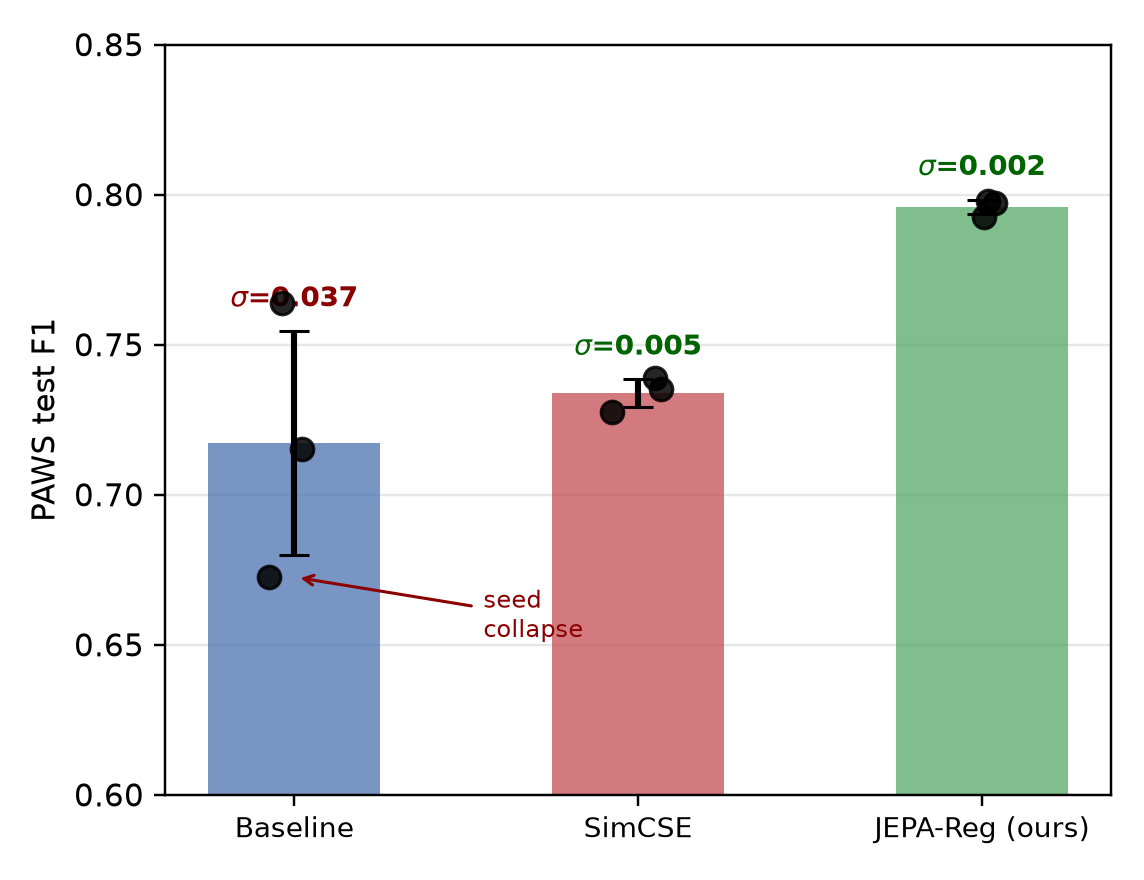
\includegraphics[width=0.82\linewidth]{figs/fig3_paws_variance}
  %% FIGURE NOTE: rescale the y-axis to 0--100 to match every table in the paper, and
  %% check the baseline annotation, which currently renders as "sigma=037" (missing
  %% decimal point; it should read 3.74 on the 0--100 scale).
  \caption{PAWS seed stability for BERT-base. Bars are mean test F1 over three seeds, error bars are $\pm 1$ standard deviation, and points are the individual per-seed values.}
  \Description{Bar chart with per-seed scatter points: the baseline has large seed spread including one collapsed seed near 0.67, SimCSE is tighter, and JEPA-Reg has both the highest mean and the smallest spread.}
  \label{fig:variance}
\end{figure}

\subsection{Main Results: RoBERTa-base}
Table~\ref{tab:roberta} reports RoBERTa-base results from the original run of the released pipeline. The absolute PAWS gain is modest because a PAWS-fine-tuned RoBERTa baseline is already near ceiling. We caution explicitly that the large $d$ reflects small within-condition variance rather than a practically large improvement; the supported claim is a small gain that is consistent across all three seeds (every JEPA-Reg seed exceeds every baseline seed).

\begin{table*}[tbp]
\caption{RoBERTa-base test F1. Conventions as in Table~\ref{tab:bert}: mean $\pm$ standard deviation over three seeds, per-seed values in parentheses for Baseline and JEPA-Reg, $d$ from pooled sample standard deviations, and $p$ from a paired $t$-test reported descriptively only.}
\label{tab:roberta}
\begin{tabular}{llllrrr}
\toprule
Dataset & Baseline & SimCSE & JEPA-Reg (ours) & $\Delta$ & $d$ & $p$ \\
\midrule
MRPC & 90.32$\pm$0.22 (90.60/90.28/90.07) & 90.75$\pm$0.30 & 90.50$\pm$0.29 (90.79/90.10/90.59) & $+0.18$ & 0.56 & 0.48 \\
PAWS & 92.09$\pm$0.10 (91.98/92.22/92.06) & 92.06$\pm$0.11 & 92.31$\pm$0.11 (92.17/92.45/92.32) & $+0.22$ & 1.75 & 0.01 \\
\bottomrule
\end{tabular}
\end{table*}

\subsection{Zero-Shot HANS Evaluation}
\label{sec:hans}
Results use the best-validation MRPC checkpoint of a single seed (42). Overall, JEPA-Reg improves HANS F1 from 61.06 to 64.02 (+2.96) at essentially unchanged accuracy (baseline 50.28 vs.\ JEPA-Reg 50.09) on this balanced benchmark. Following McCoy et al.~\cite{mccoy2019right}, Table~\ref{tab:hans} breaks accuracy down by heuristic and gold label---the diagnostic that distinguishes structural transfer from prediction-bias shifts.

\begin{table}[!htbp]
\caption{HANS accuracy by heuristic $\times$ gold label ($n$=5{,}000 per cell), single seed-42 models.}
\label{tab:hans}
\begin{tabular}{llrrr}
\toprule
Heuristic & Subcase & Baseline & SimCSE & JEPA-Reg \\
\midrule
Lex.\ overlap & entailed     & 96.46 & 97.98 & 99.92 \\
Lex.\ overlap & non-entailed & 3.28  & 1.60  & 0.34  \\
Subsequence   & entailed     & 93.82 & 95.82 & 99.34 \\
Subsequence   & non-entailed & 9.78  & 9.92  & 1.32  \\
Constituent   & entailed     & 43.56 & 49.58 & 67.18 \\
Constituent   & non-entailed & 54.80 & 47.08 & 32.42 \\
\bottomrule
\end{tabular}
\end{table}

\emph{This analysis does not support a structural-transfer interpretation.} JEPA-Reg's F1 gains arise from predicting ``entailment'' more often on overlap-heavy pairs: entailed-subcase accuracy rises on every heuristic while non-entailed accuracy falls. In zero-shot transfer, the model's improved calibration on MRPC-style distribution structure does not translate into discriminating HANS's non-entailed constructions; it translates into a stronger prior that high-overlap pairs are positive. We therefore withdraw the claim made in an earlier version of this work that HANS constituent selectivity provides behavioral evidence of structural reasoning, and report this as an honest negative result. The in-domain overlap-stratified analysis (Section~\ref{sec:overlap}), which does survive its corresponding per-class check, remains the supported behavioral evidence.

\section{Analysis}

\subsection{$\lambda$ Sensitivity}
\label{sec:lambda}
Table~\ref{tab:lambda} evaluates every $\lambda$, including the LLM-JEPA default $\lambda=1.0$, with all three seeds. These are independent sensitivity runs rather than the main-results checkpoints in Table~\ref{tab:bert}. In particular, the $\lambda=0.05$ row is a nominally matching configuration but comes from the sensitivity batch, so its $79.16\pm0.24$ PAWS value is not expected to reproduce the canonical $79.59\pm0.24$ value in Table~\ref{tab:bert}. The held-out tuning procedure selected $\lambda=0.05$ before test evaluation, whereas this table reports test-set sensitivity across fixed $\lambda$ values. With the pipeline's $\lambda$ warmup, JEPA-Reg is \emph{insensitive to $\lambda$ across $[0.05, 1.0]$} on both datasets---the PAWS means remain within a narrow range and all retain a large gain over the baseline (71.72$\pm$3.74). A control without $\lambda$ warmup at $\lambda=1.0$ also matches in mean (79.70$\pm$1.04, seeds 78.80/81.16/79.15), with a larger seed spread that we note descriptively but do not test at $n=3$. We therefore withdraw the earlier claim that the LLM-JEPA default $\lambda=1.0$ is harmful in this discriminative setting. Practically, this is good news: the method requires no careful $\lambda$ tuning, but this is a null result for $\lambda$ as a critical hyperparameter, and we report it as such.

\begin{table}[!htbp]
\caption{Sensitivity to the auxiliary-loss weight $\lambda$. Values are mean $\pm$ std over three seeds.}
\label{tab:lambda}
\begin{tabular}{lcc}
\toprule
$\lambda$ & MRPC & PAWS \\
\midrule
0.05 & 85.59$\pm$0.34 & 79.16$\pm$0.24 \\
0.10 & 85.91$\pm$0.30 & 79.45$\pm$0.52 \\
0.30 & 85.70$\pm$0.39 & 79.29$\pm$0.25 \\
0.50 & 85.84$\pm$0.27 & 79.59$\pm$0.59 \\
1.00 (LLM-JEPA default) & 85.74$\pm$0.42 & 79.58$\pm$0.45 \\
1.00, no warmup (control) & --- & 79.70$\pm$1.04 \\
\bottomrule
\end{tabular}
\end{table}

\subsection{Data Efficiency}
Figure~\ref{fig:lowresource} shows BERT-base results for 1\%--100\% of MRPC (RoBERTa was not run in the low-resource sweep). Below 25\% of the training set, the apparent F1 values are dominated by majority-class behavior rather than meaningful learning: the MRPC test set is 66.5\% positive, so an always-paraphrase predictor already obtains about 79.87 F1. The 1\%--25\% points therefore should not be interpreted as evidence of useful low-resource learning. From 50\% onward, JEPA-Reg tracks the baseline closely (at 50\%: JEPA-Reg 82.16 vs. baseline 82.29). At 100\%, the independent low-resource sweep gives 85.50 for JEPA-Reg versus 84.63 for the baseline. This is close to, but not identical to, the canonical full-data result in Table~\ref{tab:bert} (85.44 vs.\ 85.53); note that the ordering of the two conditions also differs between the two batches, which is within the run-to-run variation documented in Section~\ref{sec:implementation}. The 100\% sweep point is from a separate low-resource batch, so it is treated as a consistency check rather than a replication of the main-results checkpoint. Seed variance is not consistently smaller for JEPA-Reg in the low-resource sweep: it is smaller at 1\%, 5\%, and 100\%, but larger at 2\%, 10\%, 25\%, and 50\%. We therefore make no claim of uniform variance reduction in the low-resource regime. The useful conclusion is limited to the mid-to-full-data region, where the methods remain close in in-domain F1.

\begin{figure}[!htbp]
  \centering
  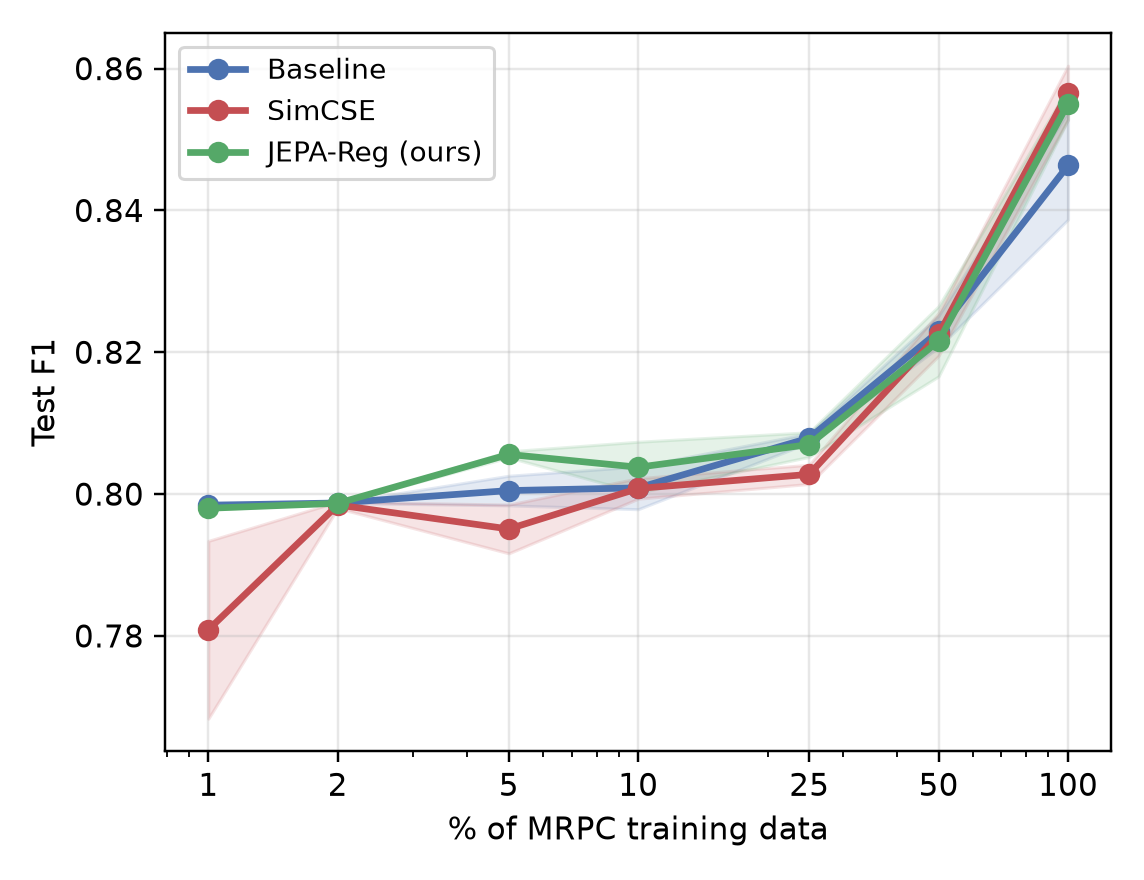
\includegraphics[width=0.85\linewidth]{figs/fig4_lowresource}
  %% FIGURE NOTE: rescale the y-axis to 0--100 to match the tables.
  \caption{BERT-base performance under different MRPC training-set sizes. Lines are means over three seeds and shaded bands are $\pm 1$ standard deviation.}
  \Description{Line chart of test F1 versus percentage of MRPC training data on a log scale; the low-data points are close to the majority-class F1 floor, while the 50 and 100 percent points show meaningful model behavior.}
  \label{fig:lowresource}
\end{figure}

\subsection{Lexical Overlap Stratification}
\label{sec:overlap}
PAWS is constructed from high-overlap pairs: in the test set, word-level Jaccard overlap has median 0.889 and minimum 0.60. Consequently, fixed bins of 0--25\% and 25--50\% overlap contain \emph{zero} examples (and 50--75\% only 84), so we stratify by empirical overlap \emph{quartiles} ($n \approx 2{,}000$ each), annotate class balance, and report per-class accuracy to separate genuine robustness from shifts in the class prior (Figure~\ref{fig:overlap}, Table~\ref{tab:overlap}).

\begin{table}[!htbp]
\caption{PAWS accuracy by Jaccard-overlap quartile. ``Base'' and ``JEPA'' are the overall accuracy of the Baseline and of JEPA-Reg; the two ``J.'' columns are JEPA-Reg's accuracy on paraphrases ($y{=}1$) and on non-paraphrases ($y{=}0$) respectively.}
\label{tab:overlap}
%% Compact settings: this table has 8 columns and overflows \columnwidth at the
%% default \tabcolsep. Do not lengthen the column headers -- the caption defines them.
\setlength{\tabcolsep}{3.5pt}
\begin{tabular}{@{}lrrrrrrr@{}}
\toprule
Quartile & $n$ & \%pos & Base & SimCSE & JEPA & J.$|_{y=1}$ & J.$|_{y=0}$ \\
\midrule
$[0.60,0.85)$ & 1980 & 42.4 & 67.5 & 69.0 & 76.9 & 85.6 & 70.5 \\
$[0.85,0.89)$ & 1927 & 46.5 & 70.5 & 71.6 & 78.9 & 89.0 & 70.1 \\
$[0.89,0.94)$ & 2091 & 47.3 & 69.8 & 72.5 & 80.9 & 90.4 & 72.4 \\
$[0.94,1.00]$ & 2002 & 40.4 & 71.0 & 74.7 & 83.3 & 92.1 & 77.3 \\
\bottomrule
\end{tabular}
\end{table}

\begin{figure}[!htbp]
  \centering
  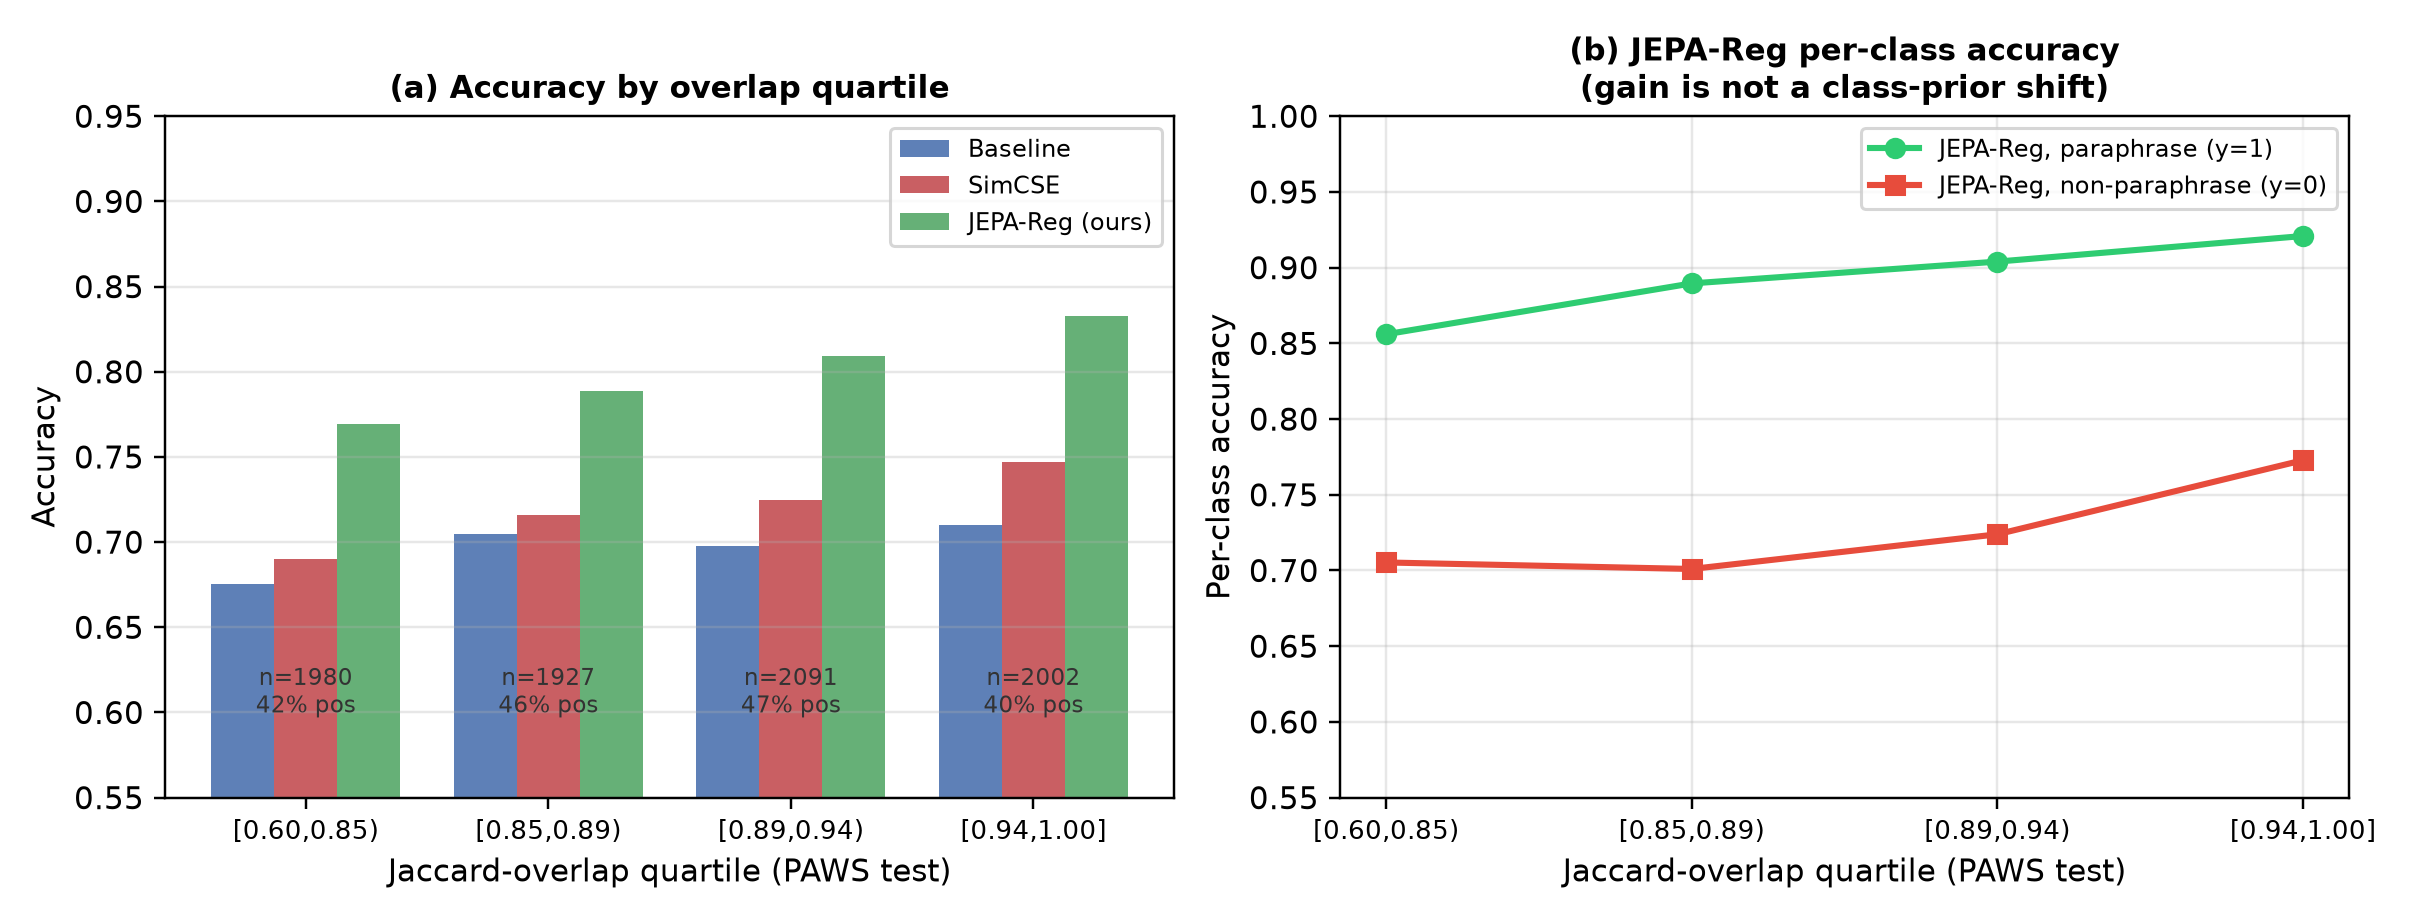
\includegraphics[width=\linewidth]{figs/fig5_overlap}
  %% FIGURE NOTE: panels (a) and (b) currently use different y-axis ranges
  %% (0.55--0.95 vs. 0--1); unify them, and rescale to 0--100 to match the tables.
  \caption{PAWS accuracy across Jaccard-overlap quartiles. (a) Overall accuracy per quartile for all three methods. (b) JEPA-Reg's per-class accuracy, which shows that the gain is not a shift in the class prior.}
  \Description{Left panel: grouped bar chart of accuracy per overlap quartile for baseline, SimCSE and JEPA-Reg, with sample size and percent positive annotated per bin; JEPA-Reg leads in every bin, with its largest lead in the highest-overlap quartile. Right panel: JEPA-Reg accuracy per class, with non-paraphrase accuracy rising from 0.71 to 0.77 across quartiles.}
  \label{fig:overlap}
\end{figure}

Two patterns support the robustness interpretation. First, JEPA-Reg's advantage over the baseline is largest in the highest-overlap quartile (+9.4 $\rightarrow$ +8.4 $\rightarrow$ +11.1 $\rightarrow$ +12.3 accuracy points); the sequence is not monotonic because the gain in the second quartile is smaller than in the first. Second, and critically, the gain is not a class-prior artifact: JEPA-Reg's accuracy on \emph{non-paraphrases}---the class a lexical-overlap heuristic gets wrong at high overlap---is 70.5, 70.1, 72.4, and 77.3 across the four quartiles. Thus it dips slightly in the second quartile before rising, rather than increasing monotonically, while the endpoint improvement from 70.5 to 77.3 shows stronger separation in the highest-overlap quartile.

\subsection{Interpreting the Behavioral Evidence}
The heuristic-level (HANS) and overlap-level (PAWS) analyses derive from the same underlying model behavior, and our per-subcase HANS analysis (Section~\ref{sec:hans}) failed to support the structural-transfer reading. The evidence that stands is in-domain: on the distribution the model is trained on, JEPA-Reg concentrates its gains exactly where lexical heuristics are most misleading and maintains them on both classes (Section~\ref{sec:overlap}). The evidence that does not stand is zero-shot: HANS gains reflect a shifted prediction prior. Decisive mechanistic evidence would require structural probing~\cite{hewitt2019structural,tenney2019bert}, which we leave to future work. Figure~\ref{fig:tsne} is included here as an exploratory visualization only; we draw no quantitative conclusions from its post-hoc clustering.
\begin{figure}[!htbp]
  \centering
  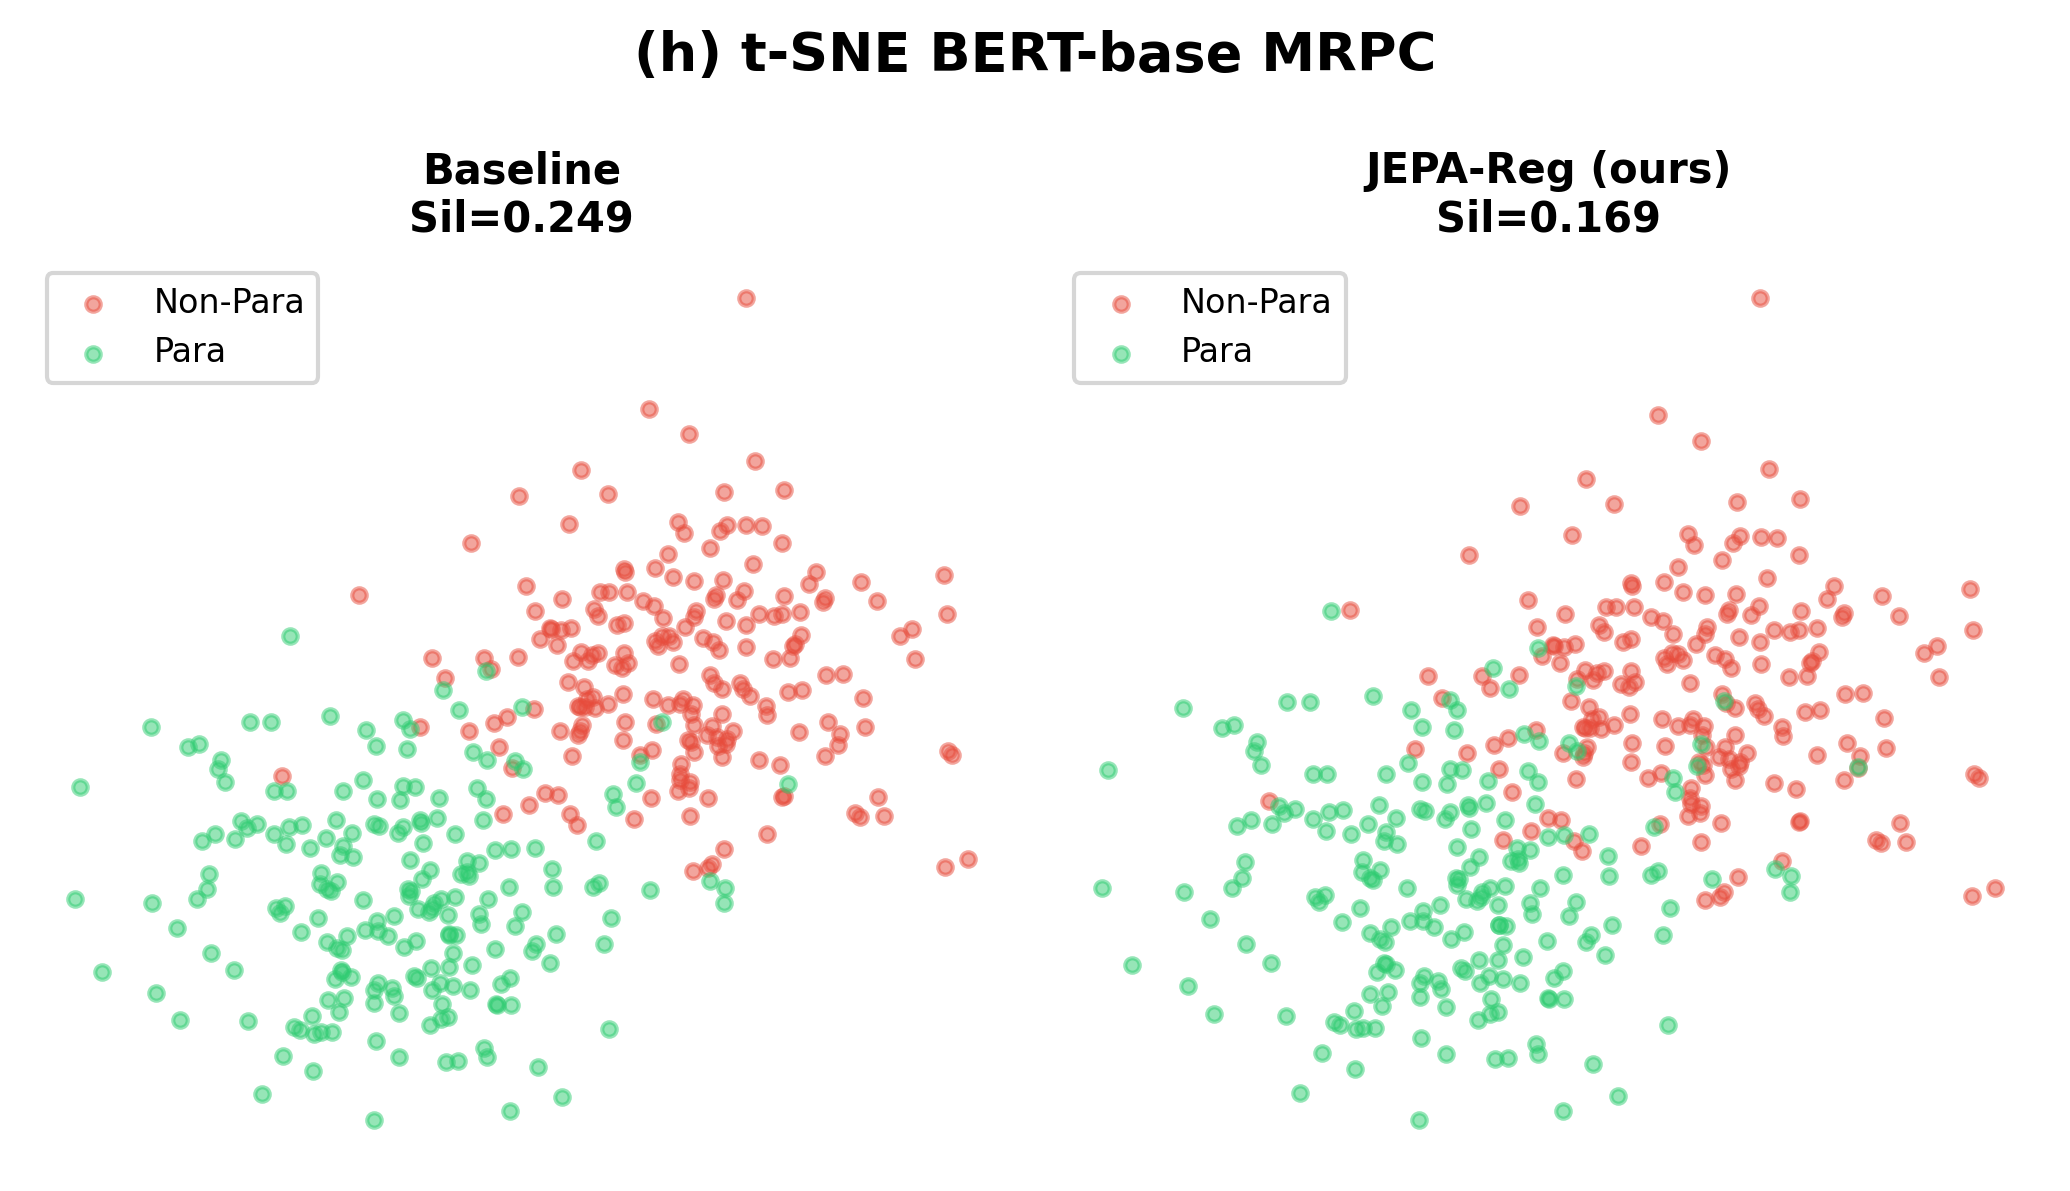
\includegraphics[width=\linewidth]{figs/fig6_tsne}
  %% FIGURE NOTE: remove the stray subplot letter "(h)" from the in-image title.
  %% TODO (author check): confirm whether the plotted vectors are the pooled sentence-pair
  %% representations (Sec. 3.1 uses mean pooling, not [CLS]); the caption below says
  %% "pooled" to stay consistent with the method.
  \caption{Exploratory t-SNE visualization of pooled sentence-pair embeddings on the MRPC test set. The silhouette score is lower for JEPA-Reg (0.169) than for the baseline (0.249); we draw no quantitative conclusion from this post-hoc clustering.}
  \Description{Three two-dimensional t-SNE scatter plots of MRPC test embeddings for baseline, SimCSE, and JEPA-Reg, with paraphrase and non-paraphrase points in different colors.}
  \label{fig:tsne}
\end{figure}

\subsection{Training Dynamics}
The final classification loss on MRPC is lower with JEPA-Reg ($0.32\pm0.01$ vs.\ $0.40\pm0.03$) with visibly smoother trajectories. These dynamics do not show \emph{why} robustness improves, but they do show that the auxiliary objective does not destabilize training in the main experimental regime; they should not be interpreted as evidence of uniformly lower seed variance across data fractions.

\subsection{Label-Conditioning Ablation and Collapse Check}
\label{sec:maskablation}
Because the label-conditioned loss (Eq.~\ref{eq:jepa}) is our main methodological departure from BYOL-style regularization, we ablate it directly: an all-pairs variant applies Eq.~(\ref{eq:pairloss}) to every training pair regardless of label (PAWS, 3 seeds; Table~\ref{tab:mask}). The positive-only row is the same nominal JEPA-Reg objective used in the main experiment, but it was rerun as part of this ablation batch; its $79.36\pm0.45$ mean should therefore be read as an ablation-batch measurement, not as a replacement for the canonical $79.59\pm0.24$ main result.

\begin{table}[!htbp]
\caption{Positive-only versus all-pairs JEPA loss on PAWS (three seeds). ``Feat.\ std'' is the mean per-dimension standard deviation of the $\ell_2$-normalized projections over the PAWS test set, and ``Eff.\ rank'' is the effective rank of their covariance matrix (the exponential of its entropy over normalized eigenvalues); both are collapse diagnostics, for which a collapsed solution would give values near zero and near one respectively.}
\label{tab:mask}
\begin{tabular}{lccc}
\toprule
Variant & PAWS F1 & Feat.\ std & Eff.\ rank \\
\midrule
Positive-only (Eq.~\ref{eq:jepa}, ours) & 79.36$\pm$0.45 & 0.0153 & 57.5 \\
All-pairs (BYOL-style) & 79.65$\pm$0.39 & 0.0167 & 50.4 \\
Baseline (no JEPA loss) & 71.72$\pm$3.74 & --- & --- \\
\bottomrule
\end{tabular}
\end{table}

Neither variant collapses (a collapsed solution would show near-zero feature variance and effective rank $\approx 1$), and the two are indistinguishable within seed noise, recovering +7.6 and +7.9 points over the baseline respectively. \emph{The honest conclusion is that the robustness gain is attributable to the predictive EMA objective itself rather than to the label mask.} We retain the positive-only form on theoretical grounds (it cannot oppose the classifier on labeled non-paraphrases, and it is the variant all other results in this paper use), but we do not claim label conditioning is empirically load-bearing on PAWS; distinguishing the two may require datasets with a higher proportion of high-overlap negatives in training.

\section{Discussion}

\subsection{Why JEPA-Reg Works}
The intended mechanism is that the label-conditioned predictive objective encourages the model to make paraphrase pairs mutually predictable in a projection space that carries no incentive to reproduce surface token patterns---especially critical for PAWS-style pairs where two sentences share almost all tokens but differ in meaning. The EMA target provides a stable reference during training. However, because the JEPA-Reg condition also uses different label smoothing from the baselines, the present experiments cannot isolate the predictive objective from that regularization difference. Because non-paraphrases are exempt from the loss, the objective never opposes the classifier's need to separate high-overlap non-paraphrases, and the per-class results in Section~\ref{sec:overlap} show that this separation is precisely where the empirical gain concentrates. We stress that Section~\ref{sec:maskablation} finds this exemption is not empirically load-bearing on PAWS, so the account above describes the intended mechanism rather than a demonstrated one.

\subsection{Comparison with Baselines}
In our setting, JEPA-Reg improves PAWS performance where SimCSE~\cite{gao2021simcse} improves it only marginally, consistent with the two methods' goals: contrastive learning separates in-batch negatives and optimizes general similarity structure, while JEPA-Reg explicitly predicts target representations for labeled paraphrases. SMART~\cite{jiang2020smart} and FreeLB~\cite{zhu2020freelb} improve robustness through embedding-space perturbations but were not evaluated here; JEPA-Reg is complementary in that it imposes a representation-level bias rather than a perturbation- or parameter-interpolation-based objective.

\subsection{QQP: No Harm, No Help}
\label{sec:qqp}
QQP does not exhibit PAWS-level overlap--label dissociation, and the baseline already performs well on our 20k-pair subsample. Pure JEPA-Reg matches the baseline (76.72$\pm$0.27 vs.\ 76.35$\pm$0.76; $d$=0.54, within noise). The Hybrid (JEPA+SimCSE) variant underperforms (75.67$\pm$0.33), indicating that the interaction of the two auxiliary objectives, not JEPA-Reg itself, caused the degradation reported in an earlier version of this work. The pattern across datasets---large improvements on PAWS, no change on MRPC or QQP---is consistent with a targeted adversarial-overlap regularizer.

\subsection{Applicability Beyond Paraphrase Detection}
\label{sec:beyond}
JEPA-Reg's mechanism---label-conditioned mutual predictability of pair members---transfers naturally to other sentence-pair classification tasks: in NLI the loss could be applied to entailment pairs, and in duplicate-question or answer-selection tasks to gold duplicates; our HANS results suggest, however, that such transfer must be trained in-domain rather than expected zero-shot. Graded-similarity tasks are a different matter: an STS-B diagnostic (zero-shot cosine similarity of MRPC-trained encoders) showed JEPA-Reg \emph{reduces} correlation with human similarity scores (Spearman $\rho$ 0.369$\rightarrow$0.362 for BERT; 0.680$\rightarrow$0.472 for RoBERTa), indicating the objective sharpens a binary decision structure rather than improving graded similarity geometry. This bounds the method's scope honestly: JEPA-Reg is a classification regularizer, not a general sentence-embedding improver.

\subsection{Limitations}
\label{sec:limitations}
First, all conclusions rest on $n=3$ seeds; per-seed values are reported throughout, effect sizes are descriptive, and no small-$p$-value claims are made---more seeds are the single most valuable robustness check. Second, we did not evaluate SMART, FreeLB, Mixout, or the debiasing methods~\cite{clark2019dont,utama2020towards}; the latter are computationally cheap at this scale and are the natural next comparison. Third, the HANS evaluation uses a single seed's checkpoint, and its per-subcase breakdown shows no evidence of zero-shot structural transfer; the method's demonstrated value is in-domain robustness. Fourth, experiments cover only 110M-parameter encoders. Fifth, RoBERTa's absolute PAWS gain is small (+0.22); the supported claim there is seed-consistency, not magnitude. Sixth, training costs 6.5$\times$ per step in our implementation (inference is unaffected). Finally, results below 25\% of MRPC are dominated by majority-class prediction rather than useful learning: the MRPC test set is 66.5\% positive and an always-paraphrase predictor already obtains 79.87 F1. We therefore do not interpret the sub-25\% points as evidence of low-resource learning. In the low-resource sweep, JEPA-Reg also does not have uniformly smaller seed variance: it is smaller at 1\%, 5\%, and 100\%, but larger at 2\%, 10\%, 25\%, and 50\%. A substantive experimental confound is that Baseline/SimCSE use 0.05 label smoothing whereas JEPA-Reg uses 0.0; this difference is not an implementation detail but a second regularization choice that could contribute to the PAWS gain and variance reduction. We did not run a matched-label-smoothing control, so the main PAWS effect should be interpreted as the effect of the complete JEPA-Reg training recipe rather than as an isolated effect of the JEPA auxiliary loss. The $\lambda$ sensitivity and label-conditioning ablations are separate rerun batches, and the low-resource sweep is likewise independent of the main-results run. Small numerical differences across these tables are therefore expected run-to-run variation; the main-results batch in Table~\ref{tab:bert} remains the canonical source for the headline comparisons.

\section{Conclusion}
We proposed JEPA-Reg, a label-conditioned JEPA-style EMA predictive auxiliary loss for BERT-based paraphrase detection. Fine-tuning on PAWS, JEPA-Reg improves BERT-base F1 by +7.9 points and reduces seed variance 15$\times$ in the main PAWS experiment, with the advantage concentrated in the most overlap-adversarial strata and maintained on both classes; RoBERTa-base shows small but seed-consistent gains. A systematic multi-seed $\lambda$ sensitivity study finds similar PAWS performance across $[0.05, 1.0]$, suggesting that the method does not require fine-grained $\lambda$ tuning. Per-subcase HANS diagnostics show that zero-shot heuristic-level gains reflect prediction-bias shifts, which we report as a negative result bounding the method's scope: JEPA-Reg is an in-domain adversarial-robustness regularizer with no inference-time overhead, not a source of transferable structural reasoning.

\FloatBarrier

\appendix

\section{PAWS Validity Diagnostics}
\label{app:paws}
Confusion matrices (seed-42 best-validation models, PAWS test; rows = gold $\{0,1\}$, columns = predicted $\{0,1\}$):
\begin{itemize}
\item Baseline: $[[2534, 1930], [494, 3042]]$ --- class-0 P/R 0.837/0.568, class-1 P/R 0.612/0.860 (bias toward the positive class).
\item SimCSE: $[[2763, 1701], [542, 2994]]$ --- class-0 P/R 0.836/0.619, class-1 P/R 0.638/0.847.
\item JEPA-Reg: $[[3245, 1219], [379, 3157]]$ --- class-0 P/R 0.895/0.727, class-1 P/R 0.721/0.893 (balanced; per-class F1 0.80/0.80).
\end{itemize}
Majority-class baseline: accuracy 55.8, positive-F1 0.0. Always-paraphrase: accuracy 44.2, F1 61.3.


\section{Reproducibility Statement}
\label{app:repro}
The code, the analysis notebook (including all revision experiments), and per-seed
result files are available at \url{https://github.com/saeefahmed/jepa-reg}.
\textbf{Hardware:} 1$\times$ NVIDIA RTX 5060 Ti (16\,GB); the full BERT-base pipeline
runs in approximately 2.5 hours.
\textbf{Software:} Python 3.14.6, PyTorch 2.13.0+cu130, Transformers 5.14.1,
Datasets 5.0.1, NumPy 2.5.1, SciPy 1.18.0, and scikit-learn 1.9.0; a complete
environment lock is included in the repository. A CUDA 12.x PyTorch build imports
successfully but cannot execute on this GPU's sm\_120 architecture.
\textbf{Seeds:} 42, 43, 44.
\textbf{Data:} MRPC, QQP, PAWS, and STS-B are obtained from the HuggingFace Hub and
HANS from its official release; no dataset files are redistributed.
\textbf{Known asymmetry:} label smoothing 0.05 (Baseline/SimCSE) vs.\ 0.0 (JEPA-Reg
classification loss), which is an acknowledged confound; no matched label-smoothing
control was run.
\textbf{Statistics:} per-seed values are reported in
Tables~\ref{tab:bert}--\ref{tab:roberta}; the exact permutation-test floor $p=0.25$
at $n=3$ is stated in Section~\ref{sec:implementation}.
\textbf{Run provenance:} the sensitivity and ablation batches of
Sections~\ref{sec:lambda}--\ref{sec:maskablation} were executed separately from the
canonical main-results batch, as documented in Section~\ref{sec:implementation}.
Trained checkpoints are omitted for size, but per-example predictions are released,
so every reported statistic and figure can be recomputed without a GPU.
\FloatBarrier
\bibliographystyle{ACM-Reference-Format}
\bibliography{references}

\end{document}
